\documentclass{beamer}
\usepackage{../common_slides}
\usepackage{pdfpages}

\title{Statistical Natural Language Processing}

\author{Alexander Rush}
\begin{document}


\begin{frame}
  \titlepage
\end{frame}

\section{Applications}

{
\setbeamercolor{background canvas}{bg=}
\includepdf[pages=3-4]{slides.pdf}
}

\begin{frame}
  \begin{center}
    \includegraphics{siri}
  \end{center}
\end{frame}

\begin{frame}
  \begin{center}
    \includegraphics[height=\textheight]{echo}
  \end{center}
\end{frame}


\begin{frame}
  \begin{center}
    \includegraphics[height=\textheight]{abelincoln}
  \end{center}
\end{frame}

% \begin{frame}{Automatic Translation}
%   \begin{center}
%     \includegraphics{translate}
%   \end{center}
% \end{frame}

\section{Scientific Challenges}

\begin{frame}
    \hspace*{-1cm} \includegraphics[width=1.2\textwidth]{../notebooks/zipf}  
\end{frame}


\begin{frame}{Challenge 1: Lexicons and Lexical Semantics}
  \textbf{Zipf' Law:}
  \begin{quote}
    The frequency of any word is inversely proportional to its rank in the frequency table.
  \end{quote}

  \begin{itemize}
  \item I.e. it is common to use rare words. 
  \item Central issue in NLP is dealing cleverly with rare words. 
  \end{itemize}
\end{frame}


\begin{frame}{(2) Structure and Probabilistic Modeling }
  \textbf{The Shannon Game:}
  \begin{quote}
    Given the last 100 words, can we predict the next one?
  \end{quote} 
  

  \texttt{The pin-tailed snipe (Gallinago stenura) is a small stocky wader. It breeds in northern Russia and migrates to spend the \_\_ } 


  \begin{itemize}
  \item Probabilistic models have become very effective at this task.
  \item Crucial for speech recognition (Jelinek), OCR, automatic translations, etc. 
  \end{itemize}



\end{frame}

\begin{frame}{(3) Compositionality and Syntax}
  \begin{quote}
    Probabilistic models give no insight into some of the basic
    problems of syntactic structure 
  \end{quote} -Chomsky

\end{frame}

\begin{frame}{(4) Document Structure and Discourse}
  Language is not merely a bag-of-words but a tool with particular properties - Harris  
  \begin{center}
    \includegraphics[width=\textwidth]{cort}
  \end{center}
\end{frame}

\begin{frame}{(5) Questions Beyond Text}
\begin{verbatim}
   The city councilmen refused the demonstrators a permit because they [feared/advocated] violence.
\end{verbatim}
\end{frame}

\begin{frame}
  \vspace{-5cm}
  
  \hspace*{-2cm}
  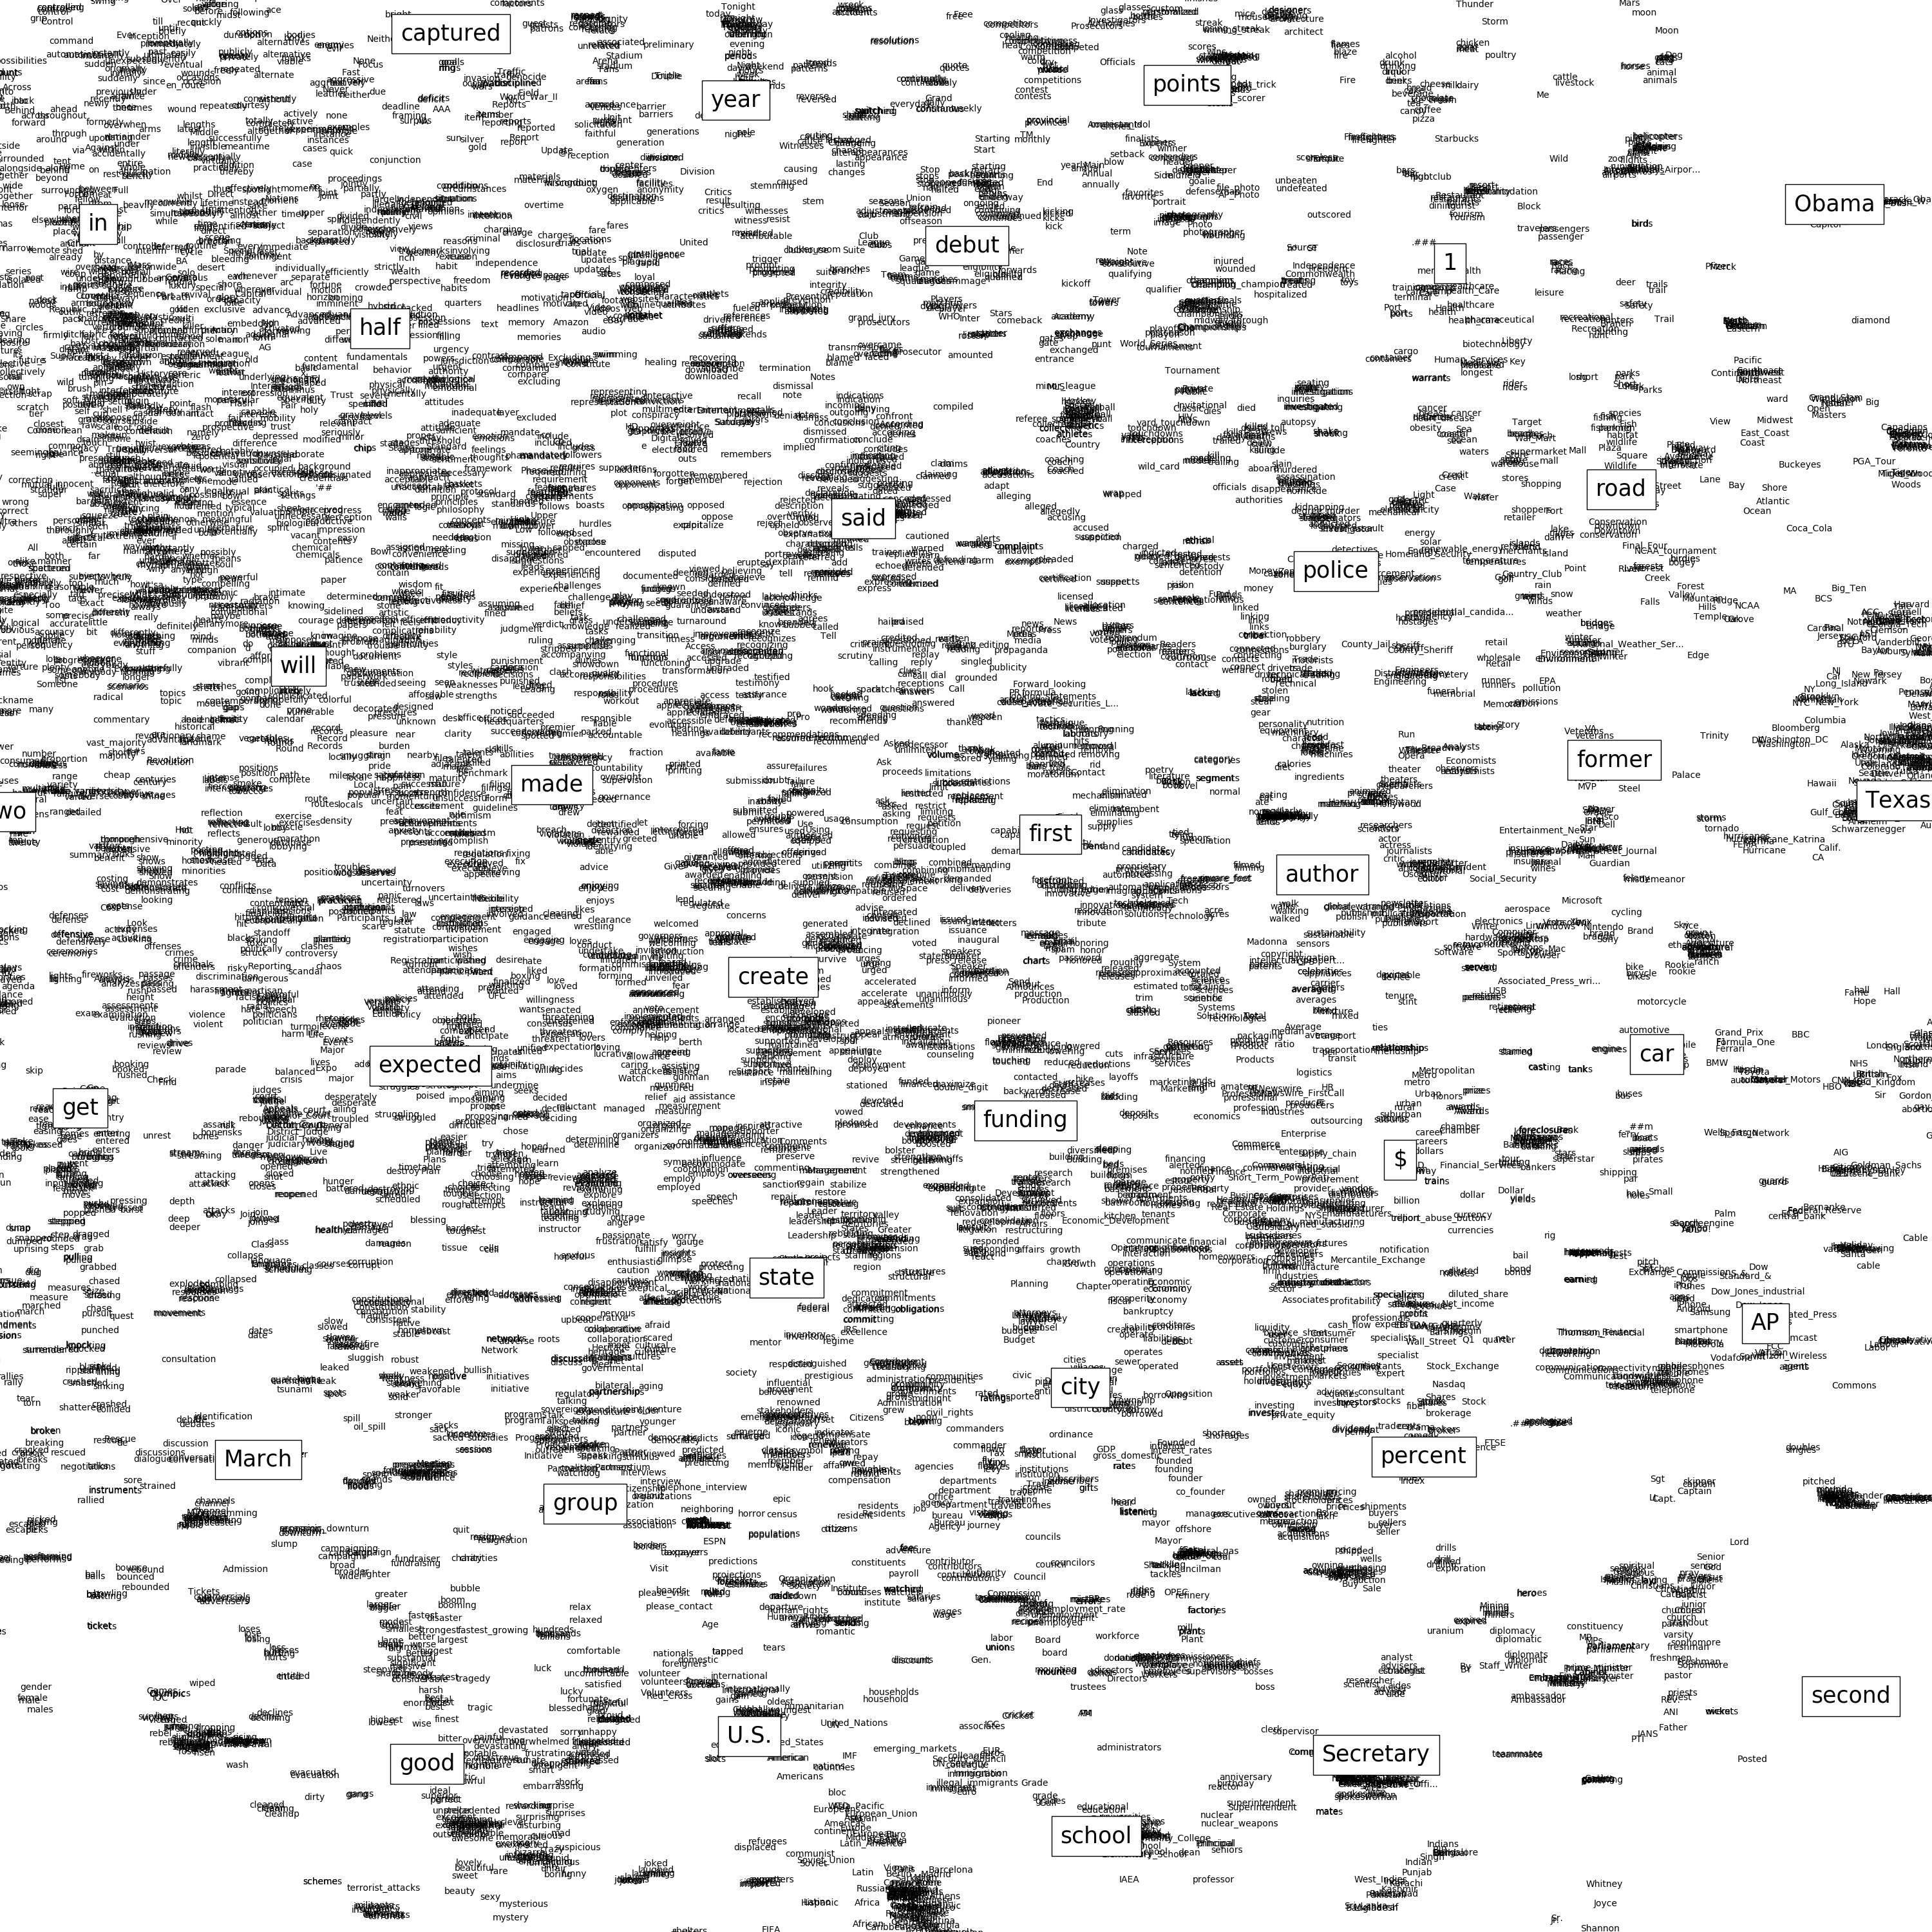
\includegraphics[width=1.5\textwidth]{../notebooks/graph}
\end{frame}

\begin{frame}
  

  
\end{frame}

\begin{frame}
  Chris Manning ``Computational Linguistics and Deep Learning''
\end{frame}

\begin{frame}
  The next big step for Deep Learning is natural language understanding, which aims to give machines the power to understand not just individual words but entire sentence and paragraphs. 
\end{frame}

\begin{frame}
  If you got a billion dollars to spend on a huge research project that you get to lead, what would you like to do? 
  
  ``I'd use the billion dollars to build a NASA-size program focusing on natural langauge processing in all of its glory (semantics, pragmatics, etc.) ... Intellectually I think that NLP is fascinating, allowing us to focus on highly structure inference programs, on issues that go to the core of `what is thought` but remain eminently practical, and on a technology that surely would make the world a better place'' 
  2014 Michael Jordan. 
\end{frame}

\begin{frame}{Intellectual Framework.}
  
\end{frame}

\begin{frame}{Computational Linguistics}
  
\end{frame}


\begin{frame}
  \includegraphics[width=\textwidth]{cell}
\end{frame}
\begin{frame}{This Class}
  Deep Learning on Language 

  \begin{itemize}
  \item 
  \end{itemize}
  
\end{frame}

\begin{frame}

\includegraphics[width=\textwidth]{../latex3}
\end{frame}


\begin{frame}
  \begin{center}
    \includegraphics[height=\textheight]{filters}
  \end{center}
\end{frame}


\begin{frame}
  \begin{center}
    \includegraphics[width=\textwidth]{lstm1}
  \end{center}
\end{frame}


\begin{frame}
  \begin{center}
    \includegraphics[width=\textwidth]{sentiment}
  \end{center}
\end{frame}


\section{Class Structure}

\begin{frame}
  
\end{frame}

\begin{frame}{Homework}
  
\end{frame}


\begin{frame}{Final Project}
  
\end{frame}



\end{document}